\documentclass[a4paper,english, 10pt, twoside]{article}
\usepackage[utf8]{inputenc}
\usepackage[T1]{fontenc}
\usepackage[english]{babel}
\usepackage{epsfig}
\usepackage{graphicx}
\usepackage{amsfonts, amssymb, amsmath}
\usepackage{listings}
\usepackage{float}
\usepackage[top=2cm, bottom=2cm, left=2cm, right=2cm]{geometry}

%opening
\title{Project 4, FYS4150}
\author{Fredrik E Pettersen\\ fredriep@student.matnat.uio.no}


\begin{document}

\maketitle


\section*{About the problem}
The aim of this project is to simulate the development of a system of spins fixed in a position in the plane. The particles can 
have spin up or down represented by the values $\pm 1$. We simulate using the simplest form of the Ising model in 2D where the energy 
of a particle is given by $E = -J\sum\limits_{\langle kl\rangle}s_{kl}$. The notation on the summation sign indicates a sum over the 
nearest neighbours of the paricle in question. $J$ is here a coupling constant which we will set equal to 1 throughout the project. 
We will also limit ourselves to using only the Metropolis algorithm with periodic boundary conditions meaning that at the boundary 
(say the right boundary) the neighbouring partice to the right of a particle at the boundary is the particle on the left boundary 
with the corresponding coordinates.

\section*{The algorithm}
The algorithm of choise here is the Metropolis algorithm combined with Monte Carlo (MC) cycles. What we end up doing in the final 
program is to run some N MC cycles and for each cycle we run trough the entire $n \times n$ grid, pick a spin at random and flip 
it. We then use the Metropolis principle to estimate wehter or not the flip is accepted. We calculate the change in energy 
$\Delta E$ caused by the flip. If the change in energy is negative the energy of the system is reduced, and the flip is accepted. 
Should the flip however increase the energy of the system we need to compare the probability of this happening to some other 
probability. In this case a random number drawn from the uniform distribution. The increase in energy for the system is not a 
non-physical move, it is simply a very unlikely one. However, this unlikeliness decreases when the temperature becomes large, 
thus more energy states will become avalible for the system at larger temperatures. We can see this very clearly if we plot the 
probability for the system to have a specific energy (or the energy distribution if we do this for all energies). We can use this 
as a sort of verification of our model, and the results can be found in the ``stability and precision'' section.

\section*{Analytic solution}
In the case where we have a lattice size of $2\times2$ we are able to find a closed form solution for all the important parameters 
in this project. We will start off by finding the energy of the system for all $2^4 = 16$ possible microstates of the system:
 
\begin{table}[H]
\centering
\begin{tabular}{|c|c|c|c|c|c|}
\hline
configuration & multiplicity ($\Omega$)& E & $|M|$ & $M$ & $M^2$\\
\hline
$\begin{matrix}\uparrow \uparrow\\ \uparrow \uparrow\end{matrix}$ & 1 & -8J & 4 & 4 & 16 \\
\hline
$\begin{matrix}\uparrow \downarrow \\ \uparrow \uparrow\end{matrix}$& 4 & 0 & 2 & 2 & 4\\
\hline
$\begin{matrix}\uparrow \uparrow \\ \downarrow \downarrow \end{matrix}$ & 4 & 0 & 0 & 0 & 0 \\
\hline
$\begin{matrix}\uparrow \downarrow  \\ \downarrow \uparrow \end{matrix}$ & 2 & 8J & 0 & 0 & 0 \\
\hline
$\begin{matrix}\uparrow \downarrow \\ \downarrow \downarrow \end{matrix}$ & 4 & 0 & 2  & -2 & 4\\
\hline
$\begin{matrix}\downarrow \downarrow  \\ \downarrow \downarrow \end{matrix}$ & 1& -8J & 4 & -4 & 16 \\

\hline
\end{tabular}
\label{table1}
\caption{All the possible spin configurations for a $2\times 2$ system of spins with periodic boudarys.}
\end{table}

From this we can find the partition function of the $2\times2$ system through the well known formula for the partition function
$$
Z = \sum\limits_E \Omega(E)e^{-\beta E} = 12 + 2e^{-8\beta J} + 2e^{8\beta J} = 4\left(3+\cosh(8\beta J)\right)
$$
We can now find the energy of the system through the relation 
\begin{align*}
 \langle E\rangle = -\frac{\partial \ln\left(Z\right)}{\partial \beta} &= -\frac{1}{4\left(3+\cosh(8\beta J)\right)}\cdot \frac{d}{d\beta}4\left(3+\cosh(8\beta J)\right)\\
 \langle E\rangle &= \frac{-8\beta J \sinh(8\beta J)}{\left(3+\cosh(8\beta J)\right)}
\end{align*}
And by differentiating this expression one more time with respect to $\beta$ we can find the heat capacity
\begin{align*}
 \langle C_V\rangle&= \frac{1}{k_BT^2}\cdot\frac{\partial^2 \ln\left(Z\right)}{\partial^2 \beta} = \frac{-(8J)^2}{k_BT^2}\cdot
 \left(\frac{\cosh(8\beta J)(3+\cosh(8\beta J)) - \sinh^2(8\beta J)}{(3+\cosh(8\beta J))^2}\right)\\
 &= \frac{-(8J)^2}{k_BT^2}\cdot\frac{3\cosh(8\beta J)}{(3+\cosh(8\beta J))^2}
\end{align*}
We can also find the expectation value of the absolute magnetization
\begin{align*}
 \langle |M|\rangle = \frac{1}{Z}\sum\limits_{i=1}^N |M_i|e^{-\beta E_i} = \frac{1}{Z}\left(2\cdot4e^{8\beta J} + 2\cdot (4\cdot 2)\right)
  = \frac{2e^{8\beta J} + 4}{3+\cosh(8\beta J)}
\end{align*}
And finally we can find the magnetic sucepitbility $\chi = \frac{\sigma_M^2}{k_BT} = \frac{\langle M^2\rangle -
\langle M \rangle^2}{k_BT}$. We find the relevant values of $\langle M^2\rangle$ and $\langle M \rangle^2$ from table 
\ref{table1}.
\begin{align*}
\chi &= \frac{1}{Z}\sum\limits_{i=1}^N M_i^2e^{-\beta E_i} -\left[\frac{1}{Z}\sum\limits_{i=1}^N M_ie^{-\beta E_i}\right]^2\\
 &= \frac{1}{Z}\left(2\cdot 16e^{8\beta J} + 2\cdot 4^2 \right) - \left[\frac{1}{Z}\left(4e^{8\beta J}-4e^{8\beta J} + 
 2-2 \right)\right]^2 = \frac{8(e^{8\beta J} + 1)}{3+\cosh(8\beta J)}
\end{align*}

\section*{Results}
As a verification of the program we can check that it reproduces the analytical results for a $2\times 2$ grid with periodic 
boundary conditions. Now, the analytical solution is for the entire system, while the program gives the results per particle, so 
we will need to divide the analytical solution by 4 to get corresponding numbers. As mentioned in the introduction we use the 
values $k_B = J = 1$ and futhermore we will do the verification for the temperature $T = 1$ where T is in units of 
$\frac{k_B T}{J}$. The results of the verification are found in table \ref{table2}

\begin{table}[H]
\centering
 \begin{tabular}{|c|c|c|c|c|}
 \hline
  - & $\langle E \rangle$ & $\langle |M|\rangle$ & $C_V$ & $\chi$  \\
\hline
  analytical & -1,995982086 & 0,998660733& 0,032075159& 3,993303776\\ \hline
  $10^5$ MC cycles & -1.99542 & 0.9984 & 0.0365311 & 3.97347\\ \hline
  $5\cdot10^5$ MC cycles & -1.99592 & 0.998659 & 0.0325315 & 3.97159\\ \hline
  $10^6$ MC cycles & -1.99606 & 0.998681 & 0.0314933 & 3.98768\\ \hline
   $5\cdot10^6$ MC cycles & -1.99599 & 0.99867  & 0.0320465 & 3.98959\\ \hline
   $10^7$ MC cycles & -1.99605 & 0.998681 & 0.0315278 & 3.99266\\ 
  \hline
 \end{tabular}
 \caption{verification of the program for a $2\times 2$ grid with increasing number of MC cycles.}
\label{table2}
\end{table}
As we can see there is a fair compliance between the analytical results and the results from the program for as few MC cycles as 
100 000. To achieve both ok results and a decent computation time I will use 1 000 000 MC cycles throughout the project.\\ \\
We would also like to see if the initial configuration of spins has a lot to say with regard to how fast the system reaches 
equilibrium. We do this for a $20 \times 20$ grid starting out with $T = 1$. 
\begin{figure}[H]
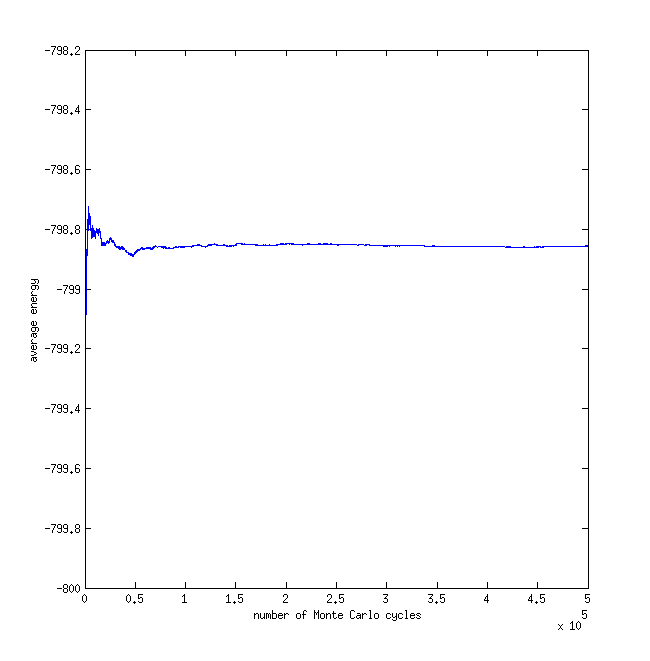
\includegraphics[scale=0.45]{energy_ordered_temp1.png}
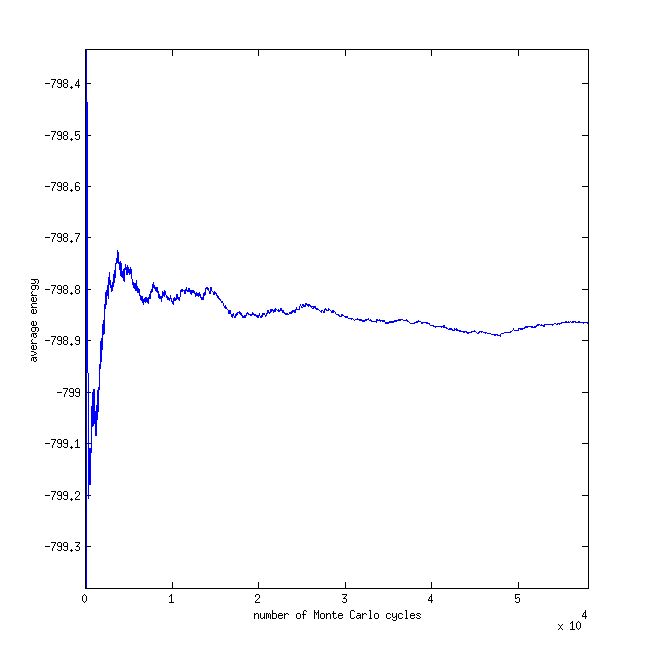
\includegraphics[scale=0.45]{energy_ordered_temp1_zoom.png}
\caption{Convergence of the total energy $20 \times 20$ grid temperature is 1, all spins pointing up initially.}
\label{energy_ordered_temp1}
\end{figure}

\begin{figure}[H]
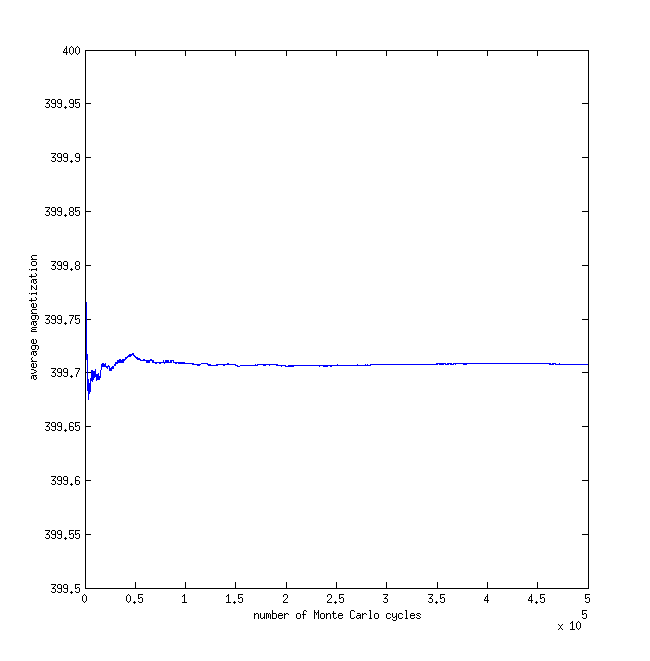
\includegraphics[scale=0.45]{magnetization_ordered_temp1.png}
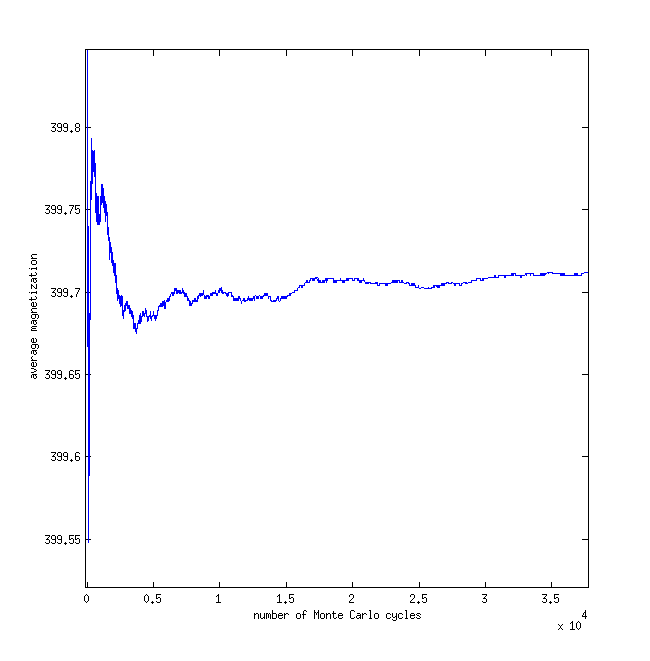
\includegraphics[scale=0.45]{magnetization_ordered_temp1_zoom.png}
\caption{Convergence of the total magnetization $20 \times 20$ grid temperature is 1, all spins pointing up initially.}
\label{magnet_ordered_temp1}
\end{figure}
In both figure \ref{energy_ordered_temp1} and \ref{magnet_ordered_temp1} the picture on the right is simply a closeup of 
the interesting part of the left picture. We can see that it takes roughly $5\cdot10^4 = 50 000$ MC cycles for the energy to 
reach equilibrium which is 10\% of the total amount of MC cycles in this run. Of course when we look at the magnetization 
at equilibrium, the starting point could not have been better. So what happens if we should start out with a random distribution. 
We can see the results in figure \ref{energy_random_temp1}. Surprisingly this seems like a much better starting point even though
the initial distribution of spins is far from the equilibrium at the relevant temperature. Figures \ref{magnet_random_temp2.4}
and \ref{both_ordered_temp2.4} show the same plots for the temperature 2.4. We can see from theese plots that it does not seem 
to matter too much which configuration we start out with. This is because there is no well defined equilibrium configuration of 
spins at this temperature. The stable (equilibrium) configuration is the random one (we can see this from the magnetization plot 
when we know that the absolute value of the magnetization is plotted). Thus every initial configuration is equally close to the 
equilibrium configuration and as we saw for $T = 1$ starting close to equilibrium means slow convergence.

\begin{figure}[H]
 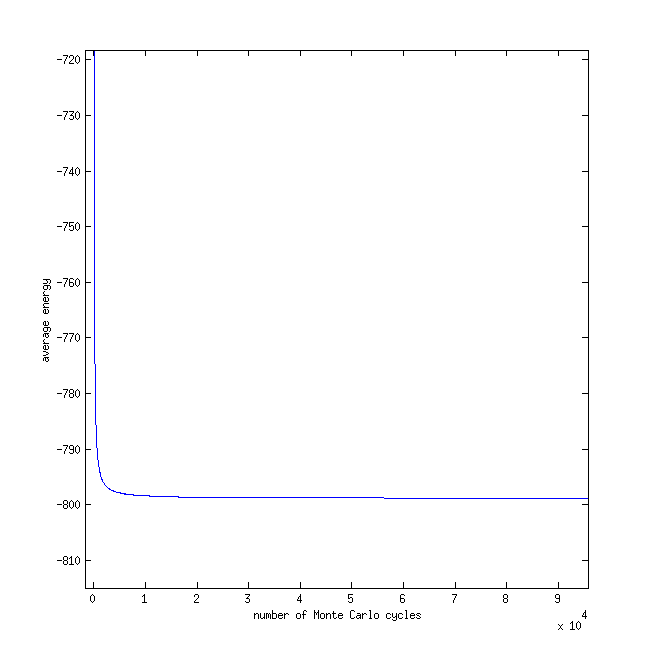
\includegraphics[scale=0.5]{energy_random_temp1_zoom.png}
 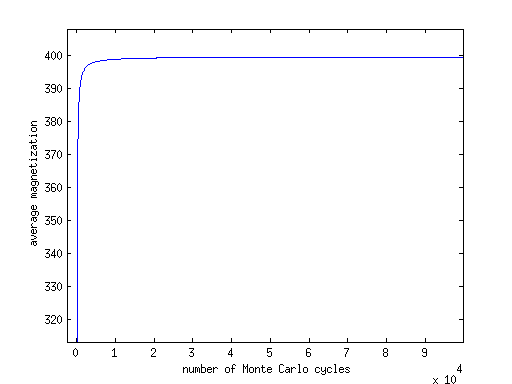
\includegraphics[scale=0.6]{magnetization_random_temp1_zoom}
 \caption{Convergence of the total energy and magnetization $20 \times 20$ grid temperature is 1,random initial configuration.}
\label{energy_random_temp1}
 \end{figure}

\begin{figure}[H]
 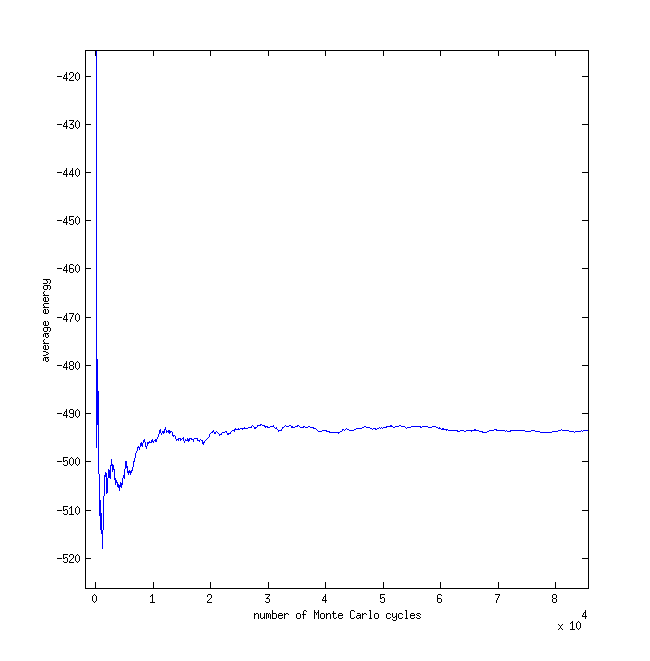
\includegraphics[scale=0.45]{energy_random_temp2dot4_zoom.png}
 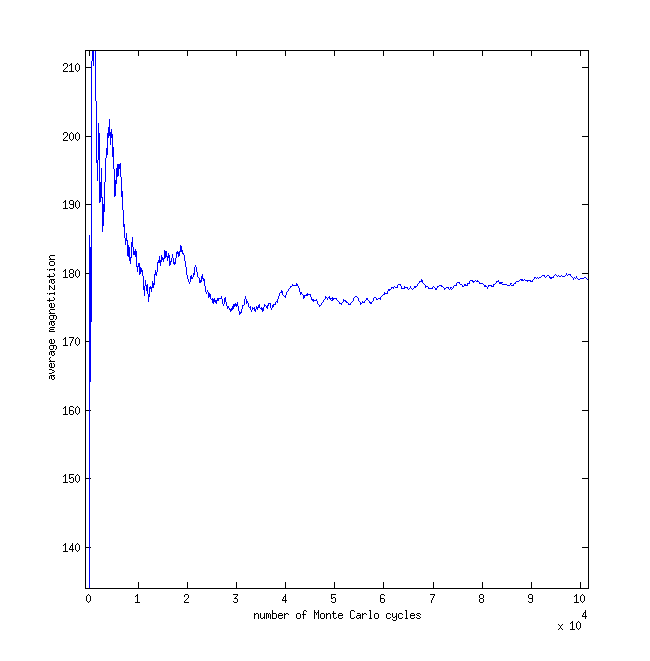
\includegraphics[scale=0.45]{magnetization_random_temp2dot4_zoom}
 \caption{Convergence of the total energy and magnetization $20 \times 20$ grid. temperature is 2.4, random initial configuration.}
\label{magnet_random_temp2.4}
 \end{figure}

\begin{figure}[H]
 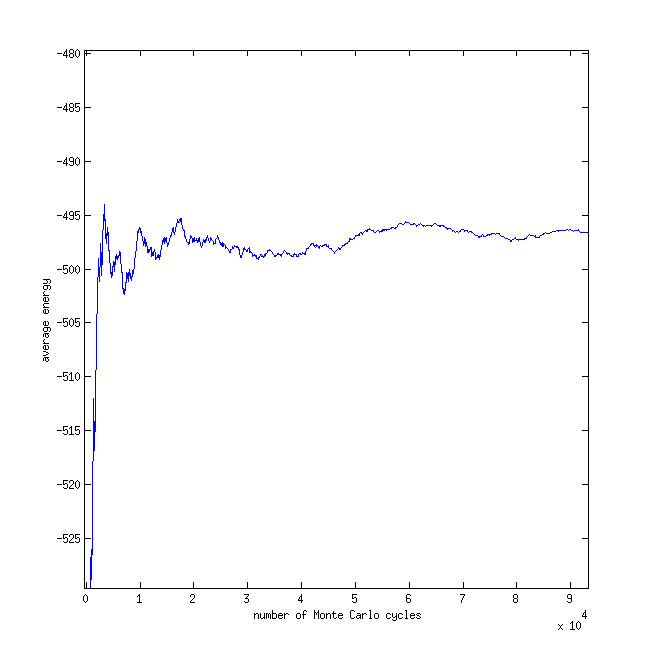
\includegraphics[scale=0.45]{energy_ordered_temp2dot4_zoom.png}
 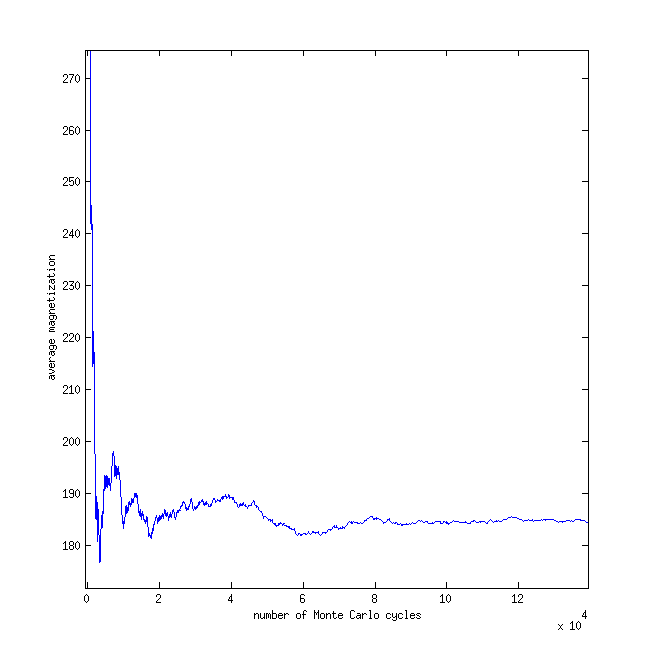
\includegraphics[scale=0.45]{magnetization_ordered_temp2dot4_zoom}
 \caption{Convergence of the total energy and magnetization $20 \times 20$ grid. Temperature is 2.4 all spins initially point up.}
\label{both_ordered_temp2.4}
 \end{figure} 

One of the things the Ising model can predict is a phase transition, and we can see this in our simplified version too, if we 
know what to look for. A (second order) phase transition is characterized by a divergence in the heat capacity and in the 
magnetic suceptibility. Unfortunately theese quantities will only truly diverge in the thermodynamic limit ($n_{spins}
\to \infty$), however we can see a discontinuity if we plot them around the critical temperature were the phase transistion 
takes place. This discontinuity will become more clear for larger grid sizes, as we can see in figure \ref{heat_capacity}. I 
realized that I have written the wrong value to file for the magnetic suceptibility (it is in fact the heat capacity) but since 
it took 8 hours to produce this data, I do not have the time to correct this... We can also see the phase transition on the 
average magnetization per particle. This will be 0 at the phase transition in the thermodynamic limit, but for finite grid sizes 
it will tend to zero more slowly as we can see in figure \ref{M_transition}.
\begin{figure}[H]
  \centering
 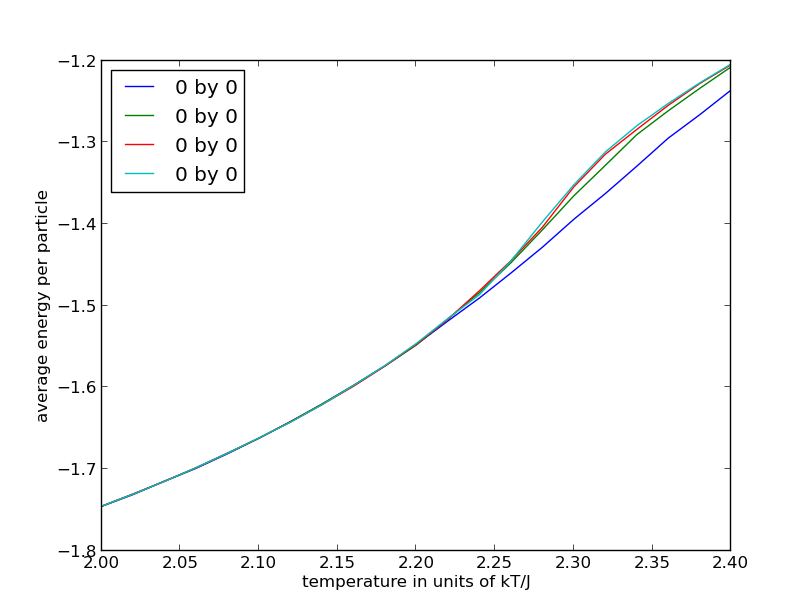
\includegraphics[scale=0.5]{energy.png}
 \caption{Energy at phase transition}
\label{E_transition}
 \end{figure} 
 
 \begin{figure}[H]
  \centering
 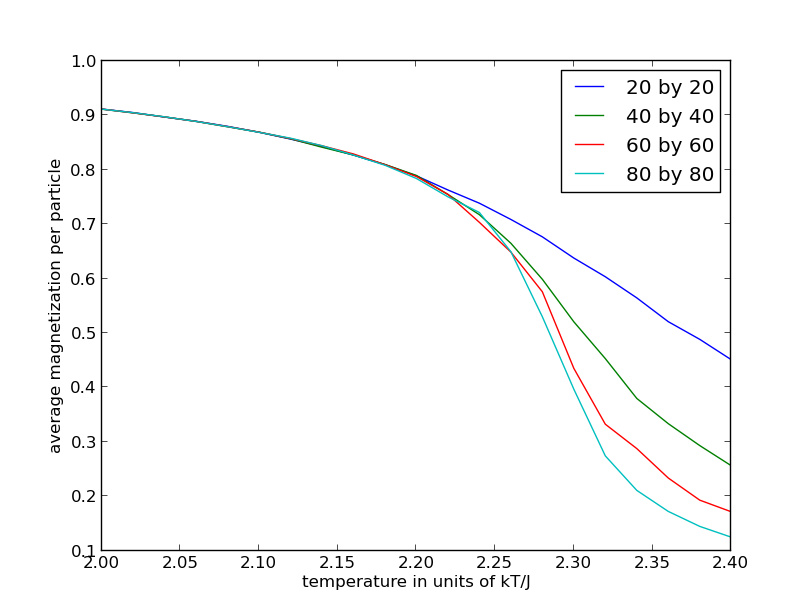
\includegraphics[scale=0.5]{magnetization.png}
 \caption{Magnetization at phase transition}
\label{M_transition}
 \end{figure} 
 
  \begin{figure}[H]
  \centering
 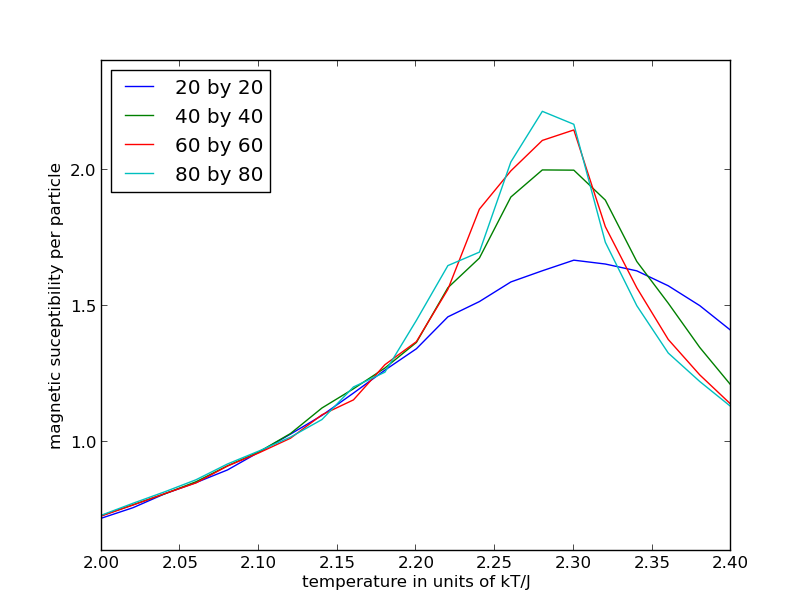
\includegraphics[scale=0.5]{magnetic_suceptibility.png}
 \caption{Magnetc sucepitbility at phase transition}
\label{magnetic_suceptibility}
 \end{figure} 
 
  \begin{figure}[H]
  \centering
 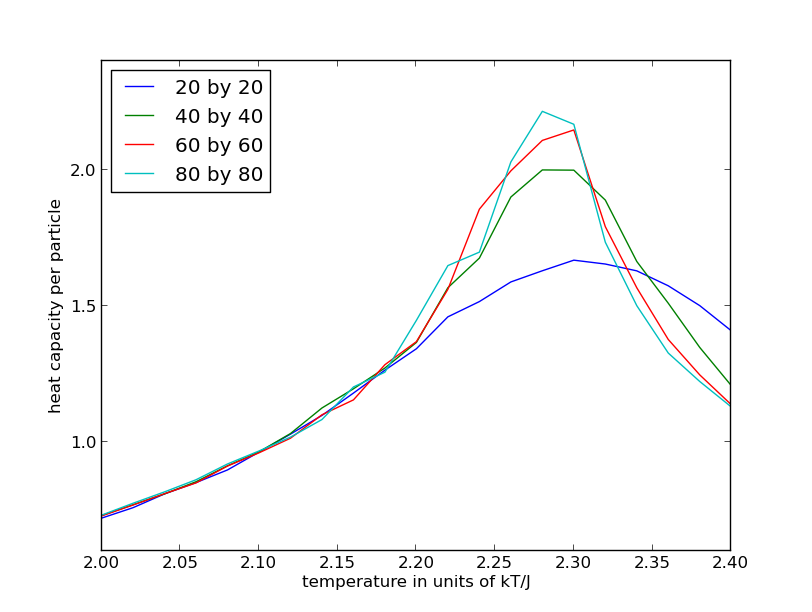
\includegraphics[scale=0.5]{heat_capacity.png}
 \caption{Heat capacity at phase transition}
\label{heat_capacity}
 \end{figure} 
\section*{Stability and precision}
All in all the Ising model with the Metropolis algorithm is a very stable, an d a very precise one. We have seen that is reproduces 
the analytical solutions for a $2\times 2$ grid nicely, and from figures \ref{probability_temp1} and \ref{probability_temp2.4} we 
see the expected behavioure that more energy-states will become avalible for the system at larger temperatures. We find the same 
behavioure in the number of accepted spin flips. For lower temperatures, very few spin configurations will be possible, and thus 
few spinflips will be accepted. For higher temperatures however, quite a lot of spin configurations are possible and more spin-flips 
will be accepted. Although I have not found a good way to illustrate this, we see the trends in figures \ref{both_accepted_flpis}.\\
The one critical 
parameter I have found is how many MC cycles we divide by when we calculate our results. If we throw away the first 10\% of the 
measurments it is absolutely vital that we only divide by 90\% of the MC cycles. Otherwise we will get completely ridiculus 
results, especially for the heat capacity, and it will take some time to debug.
\begin{figure}[H]
 \centering
 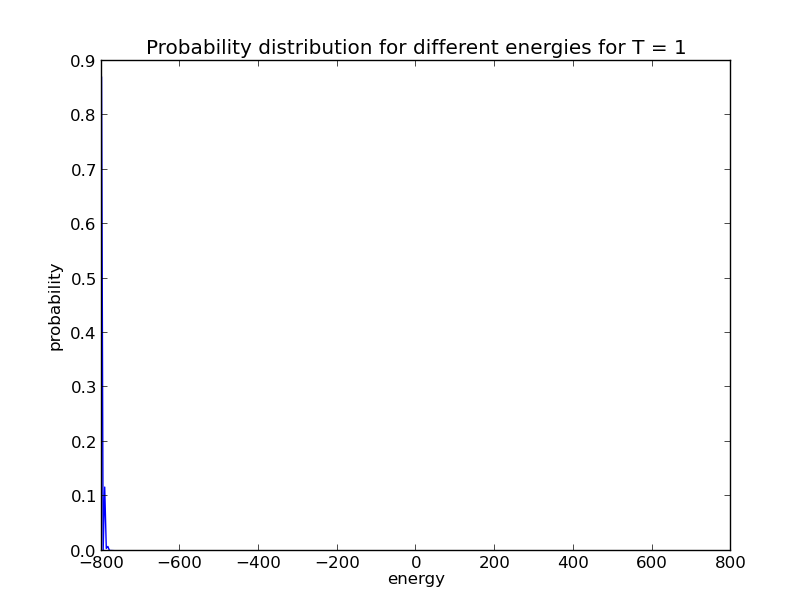
\includegraphics[scale = 0.6]{probability_temp1.png}
 \caption{Probability distribution for the total energy of the system for T = 1}
 \label{probability_temp1}
\end{figure}

\begin{figure}[H]
 \centering
 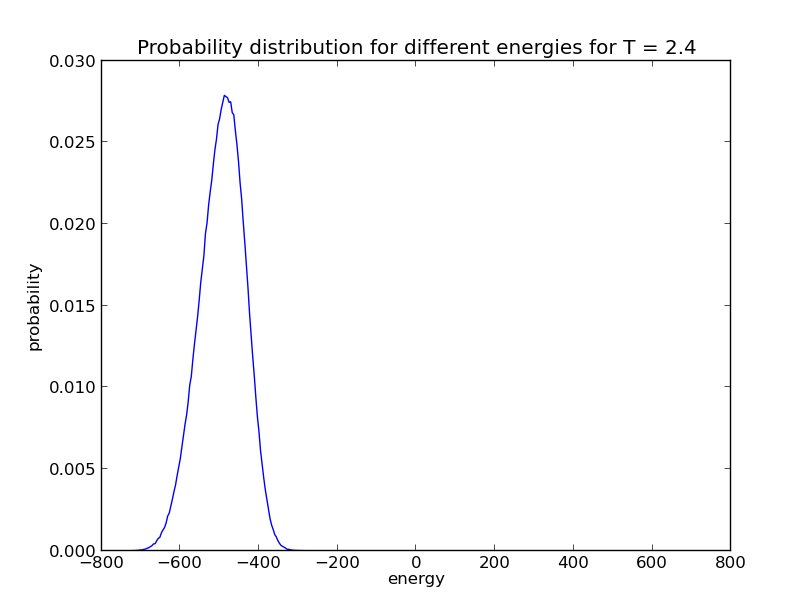
\includegraphics[scale = 0.6]{probability_temp2dot4.png}
 \caption{Probability distribution for the total energy of the system for T = 2.4}
 \label{probability_temp2.4}
\end{figure}

\begin{figure}[H]
 \centering
 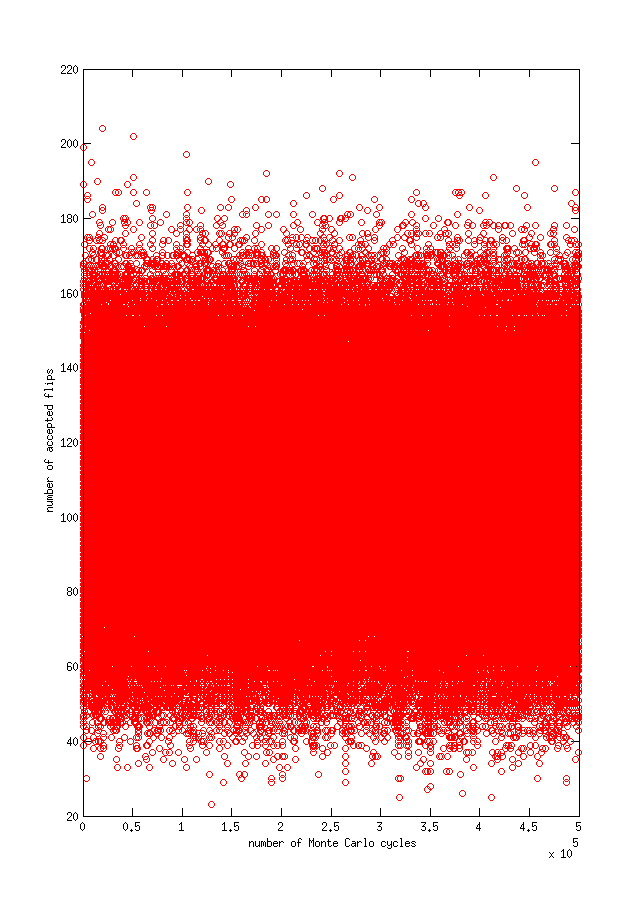
\includegraphics[scale = 0.45]{accepted_flips_temp2dot4.png}
 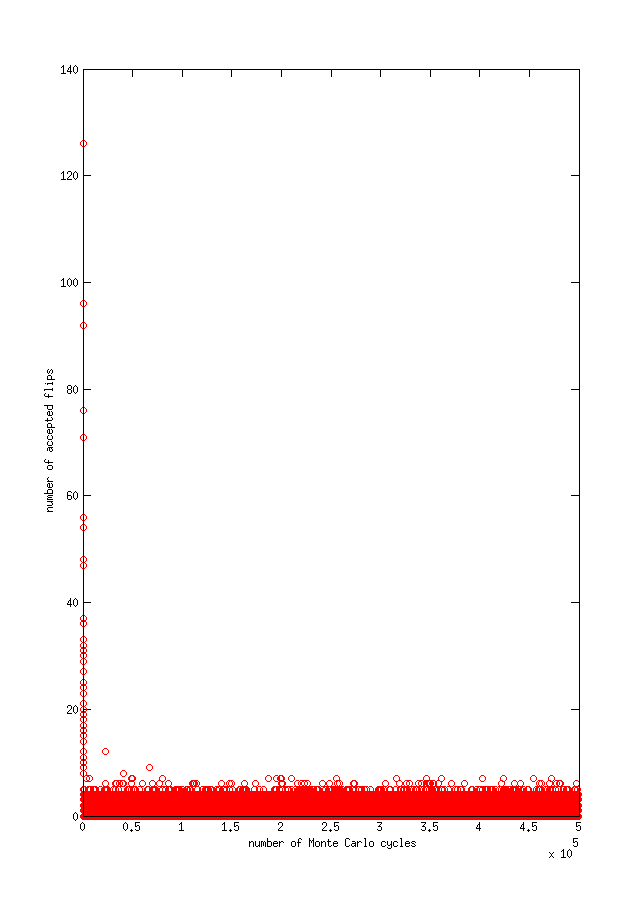
\includegraphics[scale = 0.45]{accepted_flips_temp1.png}
 \caption{Number of accepted spin flips. T = 2.4 to the left, and T = 1 on the right.}
 \label{both_accepted_flpis}
\end{figure}
\section*{Final comments}
I am not completely sure that I have understood the final part (f) of the project, but as far as I can see this is simply a question 
of finding the estimated critical temperature from figure \ref{heat_capacity} for some grid sizes, and calculate the critical 
temperature in the thermodynamic limit. We have the eqiuation
$$
T_C(L) - T_C(L=\infty) = aL^{\frac{-1}{\nu}}
$$
where $\nu = 1$. Now we happen to have 4 estimates of $T_C(L)$, but we only need two so we pick the two which should be best 
$n = 80$ and $n = 60$. This gives us
\begin{align*}
 T_C(80) - T_C(L=\infty) &= \frac{a}{80} \\
  T_C(60) - T_C(L=\infty) &= \frac{a}{60} \\
  \implies T_C(80) - \frac{a}{80} &= T_C(60) - \frac{a}{60} \\
  T_C(80) - T_C(60) = a\left(\frac{1}{80} - \frac{1}{60}\right) &\implies -0.06 = -0.004166667a \\
  a &= 14.4
\end{align*}
But this gives $T_C(L=\infty) = 2.06$  which is a much worse approximation than the one the program gives...
\end{document}
